\section{Partial Derivatives}
\begin{itemize}
    \item There are a lot of things that need to be described by several variables (e.g. temperature as a function of $x$, $y$, $z$, and time $t$)
    \begin{example}
        Suppose that:
        \begin{equation}
            f(x,y) = \frac{1}{\sqrt{ax^2-y^2}}
        \end{equation}
        The domain is when $9x^2 > y^2 \implies |y| < 3|x|$. This represents a \textit{region} in the $xy$ plane, instead of a \textit{line}. The range is when $f>0$ and occurs for $f \in (0,\infty)$.
    \end{example}
    \item Consider $z=\sqrt{a^2-x^2-y^2}$. We can define a \textbf{level curve}.
    \begin{example}
        Let $f(x,y)=xy$. Set $f=c$ such that: $y=\frac{c}{x}$. We can then plot out the function for different values of $c$:
        \begin{center}
            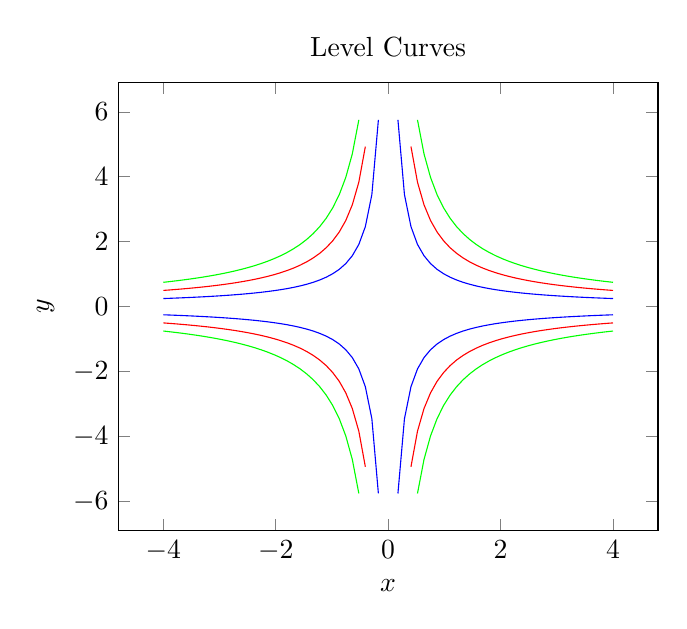
\begin{tikzpicture}
            \begin{axis}[
            legend pos=outer north east,
            title=Level Curves,
            axis lines = box,
            xlabel = $x$,
            ylabel = $y$,
            variable = t,
            trig format plots = rad,
            restrict y to domain = -6:6,
            ]
            \addplot [
                domain=-4:4,
                samples=70,
                color=blue,
                ]
                {1/x};
            \addplot [
                domain=-4:4,
                samples=70,
                color=blue,
                ]
                {-1/x};

            \addplot [
                domain=-4:4,
                samples=70,
                color=red,
                ]
                {2/x};
            \addplot [
                domain=-4:4,
                samples=70,
                color=red,
                ]
                {-2/x};

            \addplot [
                domain=-4:4,
                samples=70,
                color=green,
                ]
                {3/x};
            \addplot [
                domain=-4:4,
                samples=70,
                color=green,
                ]
                {-3/x};
            
            \end{axis}
            \end{tikzpicture}
        \end{center}
    \end{example}
    \item We can denote a function of three dimensions as $f(x,y,z)=f(\vec{x})$. For example:
    \begin{equation}
        f(x,y) = \frac{\sin x \sin y}{xy}
    \end{equation}
    Note that $f(0,0),f(x,0),f(0,y)$ are not define. But does the limit of:
    \begin{equation}
        \lim_{(x,y)\to(0,0)} \frac{\sin x \sin y}{xy} = 1
    \end{equation}
    exist?
    \begin{definition}
        Let $f$ be a function whose domain includes the region arbitrarily close to but not necessarily including $\vec{x}_0$. Then:
        \begin{equation}
            \lim_{\vec{x}\to\vec{x}_0} f(\vec{x}) = L
        \end{equation}
        if and only if for each $\epsilon > 0$, there exists a $\delta > 0$ such that if $0 < \lVert \vec{x}-\vec{x}_0 \rVert < \delta$ then $|f(\vec{x})-L| <\epsilon$.
    \end{definition}
    \begin{example}
        Again, let $f(x,y) = \frac{x^2y+y^2}{x+y^2}$. Suppose we wish to calculate:
        \begin{equation}
            \lim_{\vec{x}\to\vec{0}} f(x,y)
        \end{equation}
        Our first path is when we set $x=0$ and approach it from the $y$ axis. Then $f(0,y) = \frac{y^2}{y^2}$ whose limit:
        \begin{equation}
            \lim_{y\to 0} f(0,y) = 1
        \end{equation}
        For our second path, we approach it from the $x$ axis. Note that $f(x,0)=0/x$ such that:
        \begin{equation}
            \lim_{x\to 0} f(x,0) = 0
        \end{equation}
        For our third path, we can choose an arbitrary path, say $y=\sqrt{x}$. Then we have:
        \begin{equation}
            f(x,x^{1/2}) = \frac{1}{2}(x^{3/2}+1)
        \end{equation}
        Note that for this:
        \begin{equation}
            \lim_{x\to 0^+} f(x,x^{1/2}) = \frac{1}{2}
        \end{equation}
        We've picked three paths and they lead to different answers, so we can claim that the limit does not exist.
    \end{example}
    \begin{example}
        Suppose we have the limit $\lim_{\vec{x}\to \vec{0}} \frac{x^2y^4}{x^4+y^8}$. For our path, let's let $y=mx$. Then:
        \begin{equation}
            f(x,mx) = \frac{m^4x^6}{x^4+m^8x^8} = \frac{m^4x^2}{1+m8x^4}
        \end{equation}
        Letting $\vec{x}\to\vec{0}$ in a straight line, we get $f(x,mx)\to 0$. However, if we have a parabola and try $f(y^2,y)$, we get:
        \begin{equation}
            f(y^2,y)=\frac{y^4y^4}{y^8+y^8} = \frac{y^8}{2y^8} \to \frac{1}{2}
        \end{equation}
        Since the two paths lead to different answers, the limit does not exist.
    \end{example}
    \begin{warning}
        It's easy to determine if a function doesn't have a limit by finding counterexamples. However, it is much harder to prove a limit actually exists.
    \end{warning}
    \begin{example}
        Prove that $\lim_{\vec{x}\to\vec{0}} \frac{2xy^2}{x^2+y^2}=0$.
        \begin{enumerate}
            \item Suppose an $\epsilon > 0$ is imposed.
            \item It is required that $|f-L|<\epsilon$ or:
            \begin{align}
                \left|\frac{2xy^2}{x^2+y^2} - 0\right| &= \frac{2y^2|x|}{x^2+y^2} \\ &<\epsilon
            \end{align}
            \item when 
            \begin{equation}
                0 < \sqrt{x^2+y^2} < \epsilon
            \end{equation}
            \item Note that:
            \begin{align}
                y^2 \le x^2 + y^2 \\ 
                \frac{y^2}{y^2} \ge \frac{y^2}{x^2+y^2} \\ 
                \frac{2y^2|x|}{x^2+y^2} \le \frac{2y^2|x|}{y^2} \\ 
                &= 2|x|
            \end{align}
            Thus, we have:
            \begin{equation}
                2|x| = 2\sqrt{x^2} \le 2\sqrt{x^2+y^2} < 2\delta
            \end{equation}
            We thus choose $\delta = \frac{\epsilon}{2}$.
            \item Given $\sqrt{x^2+y^2}<\frac{\epsilon}{2}$, we have:
            \begin{equation}
                \left|\frac{2y^2x}{x^2+y^2}\right| < \epsilon
            \end{equation}
            and then:
            \begin{equation}
            \end{equation}            
        \end{enumerate}
    \end{example}
\end{itemize}